\section{ОПИСАНИЕ МОДЕЛИ ОБЪЕКТА АВТОМАТИЗАЦИИ}
\subsection{Организационная модель}

\textbf{Организационная структура} - совокупность подразделений организации и их взаимосвязей,
в рамках которой между подразделениями распределяются функциональные задачи,
определяются полномочия и ответственность руководителей и должностных лиц.

Структура предприятия устанавливается исходя из объема и содержания задач,
решаемых предприятием, направленности и интенсивности сложившихся на предприятии
информационных и документационных потоков и с учетом его организационных и материальных возможностей.

Оргструктура представляется через органограмму и такие документы, как штатное расписание,
устав организации и пр.

\textbf{Органограмма} - графическое представление структуры организации.

Основные элементы организационной диаграммы (ARIS Express 2.4i \cite{ArisExpress} Organizational chart)
представлены на рисунке~\ref{fig:ArisOrganizationalChartElements}.

\begin{figure}[!h]
    \centering
    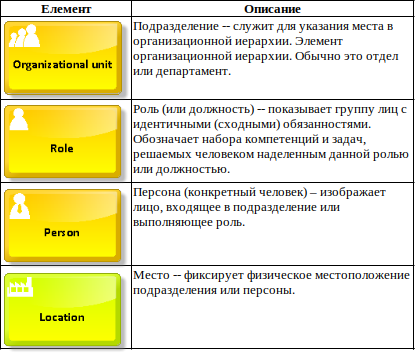
\includegraphics[width=13cm]
    {assets/ARIS/OrganizationalChart/Elements/ArisOrganizationalChartElements.png}
    \caption{Основные элементы организационной диаграммы (ARIS Express 2.4i Organizational chart)}
    \label{fig:ArisOrganizationalChartElements}
\end{figure}

Организационная модель ОА <<Косметический салон>> представлена органограммой
(см. рисунок~\ref{fig:ArisOrganizationalChart_AllOrganization})
с использованием нотации Organizational chart методологии ARIS,
а также таблицей <<Каталог организационных единиц>>
(см.~таблицу~\ref{table:ARIS_OrganizationalChart}).

\begin{figure}[!h]
    \centering
    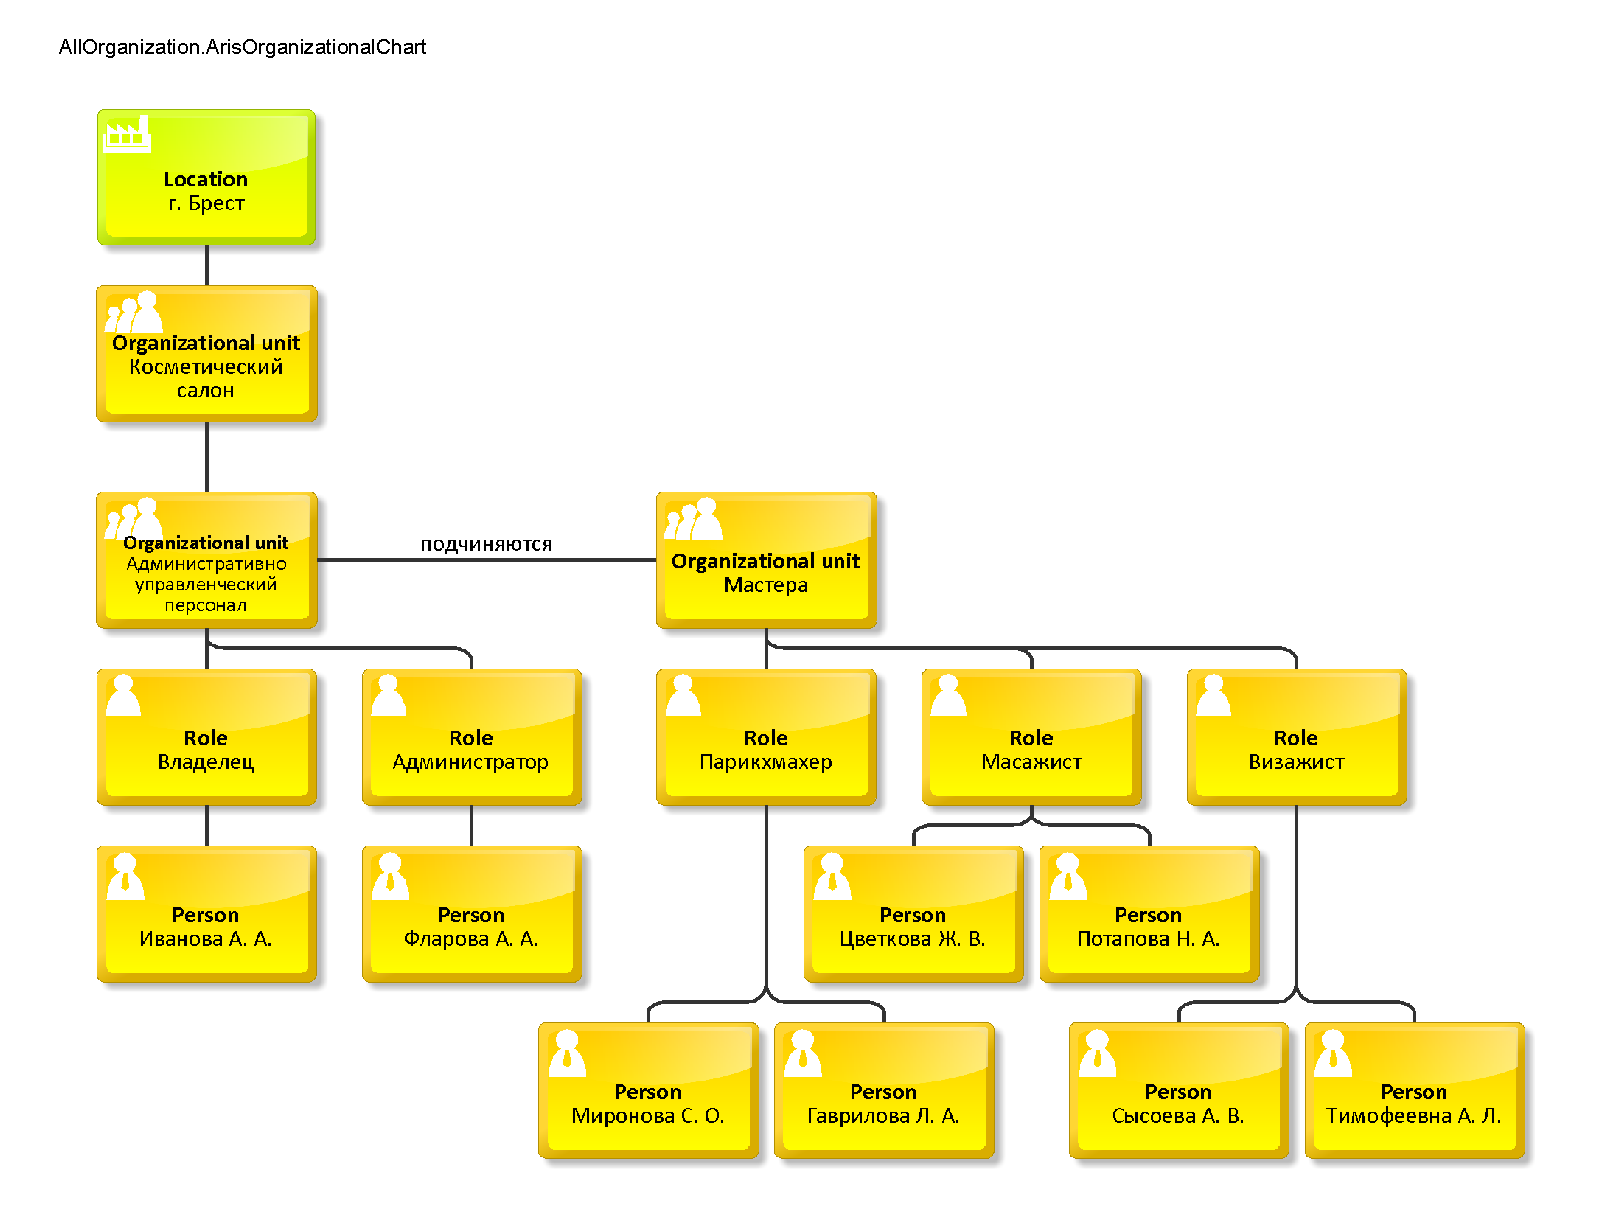
\includegraphics[width=16cm]
        {assets/ARIS/OrganizationalChart/AllOrganization.ArisOrganizationalChart.pdf}
    \caption{Органограмма ОА <<Косметический салон>>}
    \label{fig:ArisOrganizationalChart_AllOrganization}
\end{figure}

\begin{table}[h!]
    \centering

    \footnotesize

    \caption{Каталог организационых единиц}

    \label{table:ARIS_OrganizationalChart}

    \begin{tabular}{|M{1cm}|M{4cm}|M{10cm}|} 
        \hline
        \textbf{№ п/п}&\textbf{Наименование организационной единицы}&\textbf{Расшифровка}\\ \hline
    \end{tabular}

    \begin{tabular}{|p{1cm}|p{4cm}|p{10cm}|} 
        \hline
        1       &Косметический салон    &Организация по реализации услуг\\ \hline
        1.1     &Начальство             &Группа сотрудников, которые управляют организацией\\ \hline
        1.1.1   &Владелец               &Может быть председателем комиссии\\ \hline
        1.1.2   &Администратор          &Может быть председателем, так и членом инвентаризационной комиссии\\ \hline
        1.2     &Мастера                &Группа сотрудников, которые подчиняются начальству\\ \hline
        1.2.1   &Парикхмахер            &Может быть членом инвентаризационной комиссии\\ \hline
        1.2.2   &Масажист               &Может быть членом инвентаризационной комиссии\\ \hline
        1.2.3   &Визажист               &Может быть членом инвентаризационной комиссии\\ \hline
    \end{tabular}
\end{table}

Организационная модель инвентаризационная комиссия представлена органограммой
(см.~рисунок~\ref{fig:ArisOrganizationalChart_InventoryCommission})
с использованием нотации Organizational chart методологии ARIS
(ARIS Express 2.4i \cite{ArisExpress} Organizational chart),
а также таблицей <<Каталог организационных единиц инвентаризационной комиссии>>
(см.~таблицу~\ref{table:ARIS_OrganizationalChart_InventoryCommission}).

\begin{figure}[!h]
    \centering
    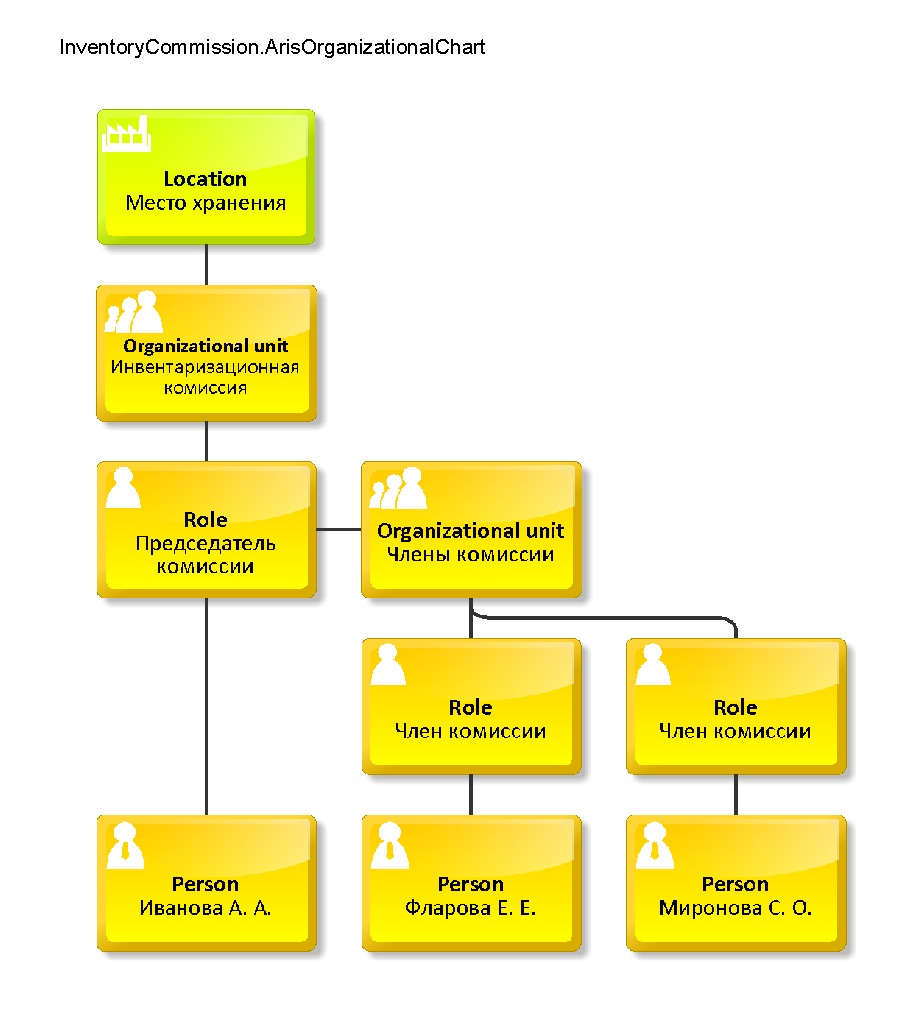
\includegraphics[height=14cm]
    {assets/ARIS/OrganizationalChart/InventoryCommission.ArisOrganizationalChart.pdf}
    \caption{Органограмма инвентаризационная комиссия}
    \label{fig:ArisOrganizationalChart_InventoryCommission}
\end{figure}

% \begin{figure}[!h]
%     \centering
%     \includegraphics[width=14cm]
%         {_docs/ОрганизационныеЕдиницы_каталог.jpg}
%     \caption{Каталог организационых единиц}
%     \label{fig:OrganizationnieEdinici_katalog}
% \end{figure}

\begin{table}[h!]
    \centering

    \footnotesize

    \caption{Каталог организационых единиц инвентаризационной комиссии}

    \label{table:ARIS_OrganizationalChart_InventoryCommission}

    \begin{tabular}{|M{1cm}|M{6cm}|M{8cm}|} 
        \hline
        \textbf{№ п/п}&\textbf{Наименование организационной единицы}&\textbf{Расшифровка}\\
    \end{tabular}

    \begin{tabular}{|p{1cm}|p{6cm}|p{8cm}|} 
        \hline
        1       &Мето хранения                  &Место, где проводится инвентаризация\\ \hline
        2       &Инвентаризационная комиссия    &Группа сотрудников\\ \hline
        3       &Председатель комиссии          &Сотрудник организации\\ \hline
        3.1     &Члены комиссии                 &Сотрудники организации\\ \hline
        3.1.1   &Член комисии                   &Сотрудник организации\\ \hline

    \end{tabular}
\end{table}

\newpage
\subsection{Функциональная модель}

\textbf{Функциональная модель объекта автоматизации} - описание его на языке выполняемых функций и их отношений.

\textbf{Функциональная структура} - структура, элементами которой являются функции,
реализуемые подразделениями предприятия, а отношениями являются связи,
обеспечивающие передачу между элементами предметов труда.
Функция – это предметно-ориентированное задание или действие,
в результате которой выполняется одна или несколько целей, стоящих перед компанией.
Функции предприятия распределяются по компонентам оргструктуры и представляют собой иерархическое дерево,
строящееся от общего к частному.
На самом верхнем уровне описываются самые сложные функции,
которые потом детализируются через свои функциональные составляющие.

Основной символ карты процессов (ARIS Express 2.4i \cite{ArisExpress} Process landscape)
изображен на рисунке~\ref{fig:ProcessLandscapeElement}.

\begin{figure}[!h]
    \centering

    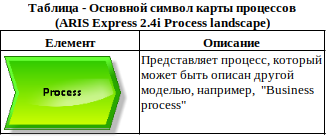
\includegraphics[width=9cm]
    {assets/ARIS/ProcessLandscape/Element/ProcessLandscapeElement.png}

    \caption{Основной символ карты процессов (ARIS Express 2.4i Process landscape)}

    \label{fig:ProcessLandscapeElement}
\end{figure}

Функциональная модель ОА <<Косметический салон>> представлена
с использованием нотации Process landscape методологии ARIS
(см.~рисунок~\ref{fig:ArisProcessLandscape}),
а также таблицей <<Каталог функций>>
(см.~рисунок~\ref{fig:ProcessLandscapeCatalog}).
Данное функциональное дерево соответствует оргструктуре.

% \begin{figure}[!h]
%     \centering
%     \includegraphics[height=8cm]
%         {_docs/ФункциональнаяМодель.png}
%     \caption{Функциональное дерево ОА "Косметический салон"}
%     \label{fig:FynctionalnayModel}
% \end{figure}

% \begin{figure}[!h]
%     \centering
%     \includegraphics[width=12cm]
%         {_docs/Функции_каталог.jpg}
%     \caption{Каталог функций}
%     \label{fig:Fynctii_katalog}
% \end{figure}

\begin{figure}[!h]
    \centering

    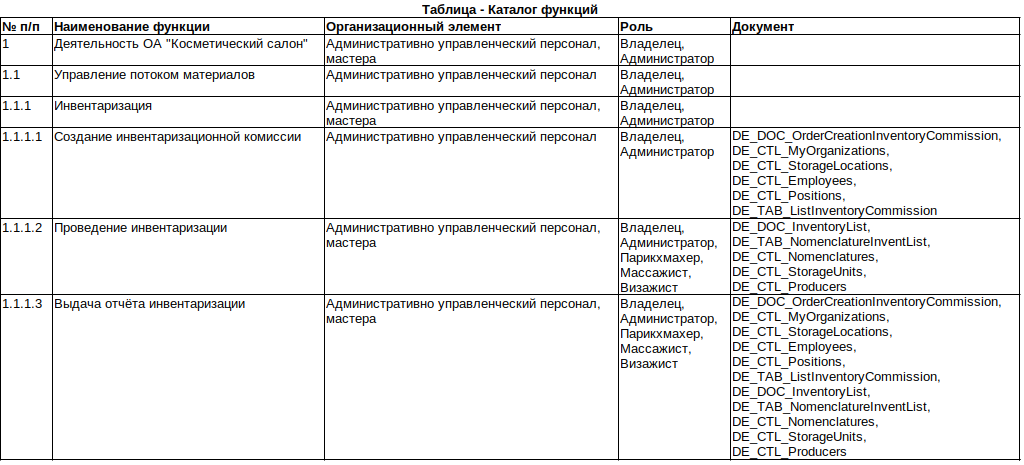
\includegraphics[width=16cm]
    {assets/ARIS/ProcessLandscape/Catalog/ProcessLandscapeCatalog.png}

    \caption{Функциональное дерево ОА "Косметический салон"}

    \label{fig:ProcessLandscapeCatalog}
\end{figure}

\begin{figure}[!h]
    \centering

    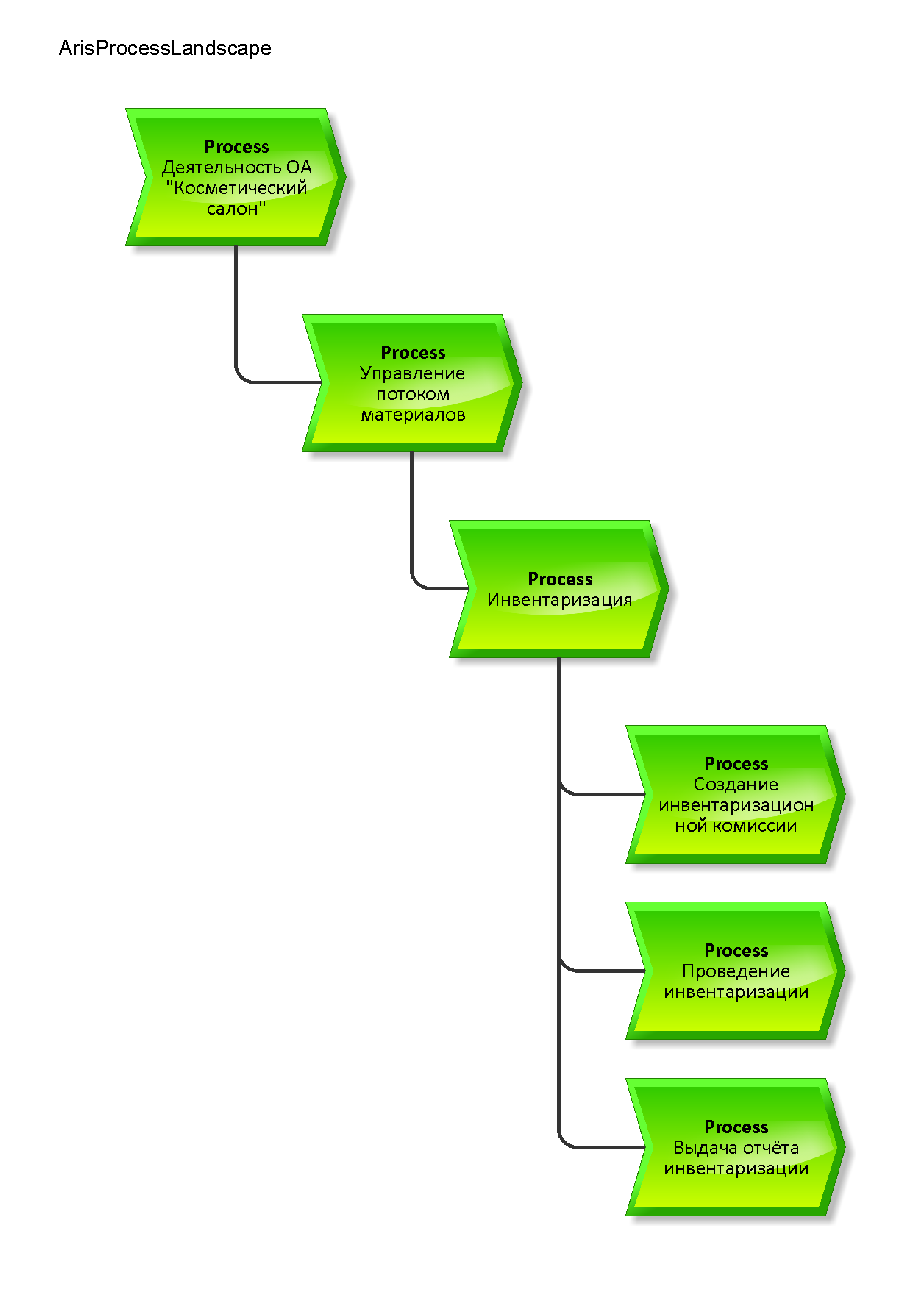
\includegraphics[width=16cm]
    {assets/ARIS/ProcessLandscape/ArisProcessLandscape.pdf}

    \caption{Функциональное дерево ОА <<Косметический салон>>}

    \label{fig:ArisProcessLandscape}
\end{figure}

\newpage
\subsection{Информационная модель}
Информационная модель - модель объекта, представленная в виде информации,
описывающей существенные для данного рассмотрения параметры и переменные величины объекта,
связи между ними, входы и выходы объекта и позволяющая путём подачи на модель информации об изменениях
входных величин моделировать возможные состояния объекта.

Информационная модель ОА <<Инвентаризация>> для ИС <<Косметический салон>> включает в себя следующие документы:

\begin{itemize}
    \item справочные документы (см.~таблицу~\ref{table:CPR_katalog});
    \item оперативные документы (см.~таблицу~\ref{table:DOC_katalog});
    \item отчётные документы (см.~таблицу~\ref{table:OTC_katalog}).
\end{itemize}

% Справочные документы представлены в <<Каталоге справочных документов>> .

\begin{table}[h!]
    \centering

    \footnotesize

    \caption{Каталог справочных документов}

    \label{table:CPR_katalog}

    \begin{tabular}{|M{1cm}|M{6cm}|M{8cm}|} 
        \hline
        \textbf{№ п/п}&\textbf{Идентификатор документа}&\textbf{Наименование документа}\\ \hline
    \end{tabular}

    \begin{tabular}{|M{1cm}|p{6cm}|p{8cm}|} 
        \hline
        1   &DE\_CTL\_Nomenclature      &Номенклатура\\ \hline
        2   &DE\_CTL\_Employees         &Сотрудники\\ \hline
        3   &DE\_CTL\_Positions         &Должности \\ \hline
        4   &DE\_CTL\_StorageUnits      &Единицы хранения\\ \hline
        5   &DE\_CTL\_MyOrganizations   &Мои организации\\ \hline
        6   &DE\_CTL\_Producers         &Производители\\ \hline
        7   &DE\_CTL\_StorageLocations  &Места хранения\\ \hline
    \end{tabular}
\end{table}

% \begin{figure}[!h]
%     \centering
%     \includegraphics[width=14cm]
%         {_docs/СП_каталог.jpg}
%     \caption{Каталог справочных документов}
%     \label{fig:CP_katalog}
% \end{figure}

% Оперативные документы представлены в <<Каталоге оперативных документов>> .

\begin{table}[h!]
    \centering

    \footnotesize

    \caption{Каталог оперативных документов}

    \label{table:DOC_katalog}

    \begin{tabular}{|M{1cm}|M{6cm}|M{8cm}|} 
        \hline
        \textbf{№ п/п}&\textbf{Идентификатор документа}&\textbf{Наименование документа}\\ \hline
    \end{tabular}

    \begin{tabular}{|M{1cm}|p{6cm}|p{8cm}|} 
        \hline
        1   &DE\_DOC\_OrderCreationInventory Commission &Приказ о создании инвентаризационной комиссии\\ \hline
        2   &DE\_DOC\_InventoryList                     &Инвентаризационная опись\\ \hline
    \end{tabular}
\end{table}

% \begin{figure}[!h]
%     \centering
%     \includegraphics[width=14cm]
%         {_docs/ОП_каталог.jpg}
%     \caption{Каталог оперативных документов}
%     \label{fig:OP_katalog}
% \end{figure}

% Отчётные документы представлены в <<Каталоге отчётных документов>> .

\begin{table}[h!]
    \centering

    \footnotesize

    \caption{Каталог отчётов}

    \label{table:OTC_katalog}

    \begin{tabular}{|M{1cm}|M{6cm}|M{8cm}|} 
        \hline
        \textbf{№ п/п}&\textbf{Идентификатор документа}&\textbf{Наименование документа}\\ \hline
    \end{tabular}

    \begin{tabular}{|M{1cm}|p{6cm}|p{8cm}|} 
        \hline
        1   &DE\_REP\_InventoryAct  &Акт об инвентаризации\\ \hline
    \end{tabular}
\end{table}

% \begin{figure}[!h]
%     \centering
%     \includegraphics[width=14cm]
%         {_docs/ОТ_каталог.jpg}
%     \caption{Каталог отчётных документов}
%     \label{fig:OT_katalog}
% \end{figure}

\newpage

\subsubsection{Справочный документ <<Номенклатура>>}

Справочник <<Номенклатура>> - содержит информацию о материалах.
Документ представлен в виде словаря данных (см.~рисунок~\ref{fig:InformationalModel_DE_CTL_Nomenclatures}).
%и макета (см.~рисунок~\ref{fig:CP_Nomenkl_maket}).

\begin{figure}[!h]
    \centering
    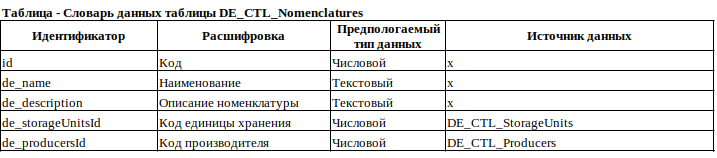
\includegraphics[width=16cm]
    {assets/InformationalModel/DE_CTL_Nomenclatures.png}
    \caption{Словарь данных справочника <<Номенклатура>>}
    \label{fig:InformationalModel_DE_CTL_Nomenclatures}
\end{figure}

% \begin{table}[h!]
%     \centering

%     \scriptsize

%     \caption{Словарь данных справочника <<Номенклатура>>}

%     \label{table:CPR_Nomenklatura_tipi}

%     \begin{tabular}{|M{0.7cm}|M{3.1cm}|M{5cm}|M{2cm}|M{5cm}|} 
%         \hline
%         \textbf{№ п/п}&\textbf{Идентификатор}&\textbf{Наименование}&\textbf{Предполага-емый тип данных}&\textbf{Источник данных}\\ \hline
%     \end{tabular}

%     \begin{tabular}{|M{0.7cm}|p{3.1cm}|p{5cm}|p{2cm}|p{5cm}|} 
%         \hline
%         1   &id&Код&N16&\\ \hline
%         2   &de\_name&Наиманование номенклатуры&C64&\\ \hline
%         3   &de\_description&Единица хранения&N16&СПР\_ЕдиницыХранения\\ \hline
%         4   &de\_storageUnitId&Производитель номенклатуры&N16&СПР\_Производители\\ \hline
%         5   &de\_producerId&Описание номенклатуры&C1024&\\ \hline
%     \end{tabular}
% \end{table}

% \begin{figure}[!h]
%     \centering
%     \includegraphics[width=14cm]
%         {_docs/СП_Номенкл_типы.jpg}
%     \caption{Словарь данных справочника <<Номеклатура>>}
%     \label{fig:CP_Nomenkl_tipi}
% \end{figure}

% \begin{figure}[!h]
%     \centering
%     \includegraphics[]
%         {_docs/СП_Номенкл_макет.jpg}
%     \caption{Макет справочника <<Номеклатура>>}
%     \label{fig:CP_Nomenkl_maket}
% \end{figure}

\subsubsection{Справочный документ <<Сотрудники>>}

Справочник <<Сотрудники>> - содержит информацию о сотрудниках.
Документ представлен в виде словаря данных (см.~рисунок~\ref{fig:InformationalModel_DE_CTL_Employees}).
%и макета (рисунок~\ref{fig:CP_Sotr_maket}).

\begin{figure}[!h]
    \centering
    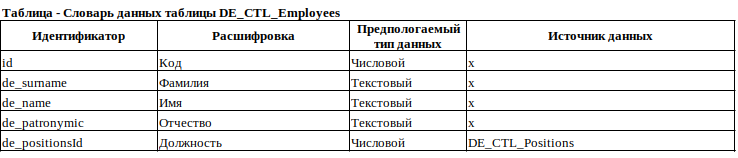
\includegraphics[width=16cm]
    {assets/InformationalModel/DE_CTL_Employees.png}
    \caption{Словарь данных справочника <<Сотрудники>>}
    \label{fig:InformationalModel_DE_CTL_Employees}
\end{figure}

% \begin{table}[h!]
%     \centering

%     \scriptsize

%     \caption{Словарь данных справочника <<Сотрудники>>}

%     \label{table:CPR_Sotrydniki_tipi}

%     \begin{tabular}{|M{0.7cm}|M{3.1cm}|M{5cm}|M{2cm}|M{5cm}|} 
%         \hline
%         \textbf{№ п/п}&\textbf{Идентификатор}&\textbf{Наименование}&\textbf{Тип данных и значность}&\textbf{Источник данных}\\ \hline
%     \end{tabular}

%     \begin{tabular}{|M{0.7cm}|p{3.1cm}|p{5cm}|p{2cm}|p{5cm}|} 
%         \hline
%         1&id&Код&N16&\\ \hline
%         2&Фамилия&Фамилия сотрудника&C32&\\ \hline
%         3&Имя&Имя сотрудника&C32&\\ \hline
%         4&Отчество&Отчество сотрудника&C32&\\ \hline
%         5&ДолжностиСотру дникаId&Должность сотрудника&N16&СПР\_ДолжностиСотрудника\\ \hline
%     \end{tabular}
% \end{table}

% \begin{figure}[!h]
%     \centering
%     \includegraphics[width=14cm]
%         {_docs/СП_Сотр_типы.jpg}
%     \caption{Словарь данных справочника <<Сотрудники>>}
%     \label{fig:CP_Sotr_tipi}
% \end{figure}

% \begin{figure}[!h]
%     \centering
%     \includegraphics[]
%         {_docs/СП_Сотр_макет.jpg}
%     \caption{Макет справочника <<Сотрудники>>}
%     \label{fig:CP_Sotr_maket}
% \end{figure}

% \newpage

\subsubsection{Справочный документ <<Должности>>}

Справочник <<Должности>> - содержит перечисления должностей.
Документ представлен в виде словаря данных (см.~рисунок~\ref{fig:DE_CTL_Positions}).
%и макета (рисунок~\ref{fig:CP_DoljnCotr_maket}).

\begin{figure}[!h]
    \centering
    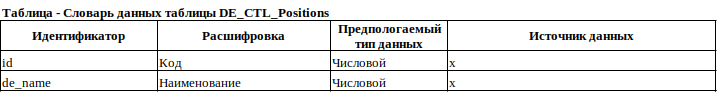
\includegraphics[width=16cm]
    {assets/InformationalModel/DE_CTL_Positions.png}
    \caption{Словарь данных справочника <<Должности>>}
    \label{fig:DE_CTL_Positions}
\end{figure}

% \begin{table}[h!]
%     \centering
% 
%     \scriptsize
% 
%     \caption{Словарь данных справочника <<Должности сотрудника>>}
% 
%     \label{table:CPR_DoljnostiSotrydnika_tipi}
% 
%     \begin{tabular}{|M{0.7cm}|M{3.1cm}|M{5cm}|M{2cm}|M{5cm}|} 
%         \hline
%         \textbf{№ п/п}&\textbf{Идентификатор}&\textbf{Наименование}&\textbf{Тип данных и значность}&\textbf{Источник данных}\\ \hline
%     \end{tabular}
% 
%     \begin{tabular}{|M{0.7cm}|p{3.1cm}|p{5cm}|p{2cm}|p{5cm}|} 
%         \hline
%         1&id&Код&N16&\\ \hline
%         2&Наименование&Должность сотрудника&C64&\\ \hline
%     \end{tabular}
% \end{table}

% \begin{figure}[!h]
%     \centering
%     \includegraphics[width=14cm]
%         {_docs/СП_ДолжнСотр_типы.jpg}
%     \caption{Словарь данных справочника <<Должности сотрудника>>}
%     \label{fig:CP_DoljnCotr_tipi}
% \end{figure}

% \begin{figure}[!h]
%     \centering
%     \includegraphics[]
%         {_docs/СП_ДолжнСотр_макет.jpg}
%     \caption{Макет справочника <<Должности сотрудника>>}
%     \label{fig:CP_DoljnCotr_maket}
% \end{figure}

% \newpage

\subsubsection{Справочный документ <<Единицы хранения>>}

Справочник <<Единицы хранения>> - содержит перечисление единиц хранения.
Документ представлен в виде словаря данных (см.~рисунок~\ref{fig:InformationalModel_DE_CTL_StorageUnits}).
%и макета (рисунок~\ref{fig:CP_EdXran_maket}).

\begin{figure}[!h]
    \centering
    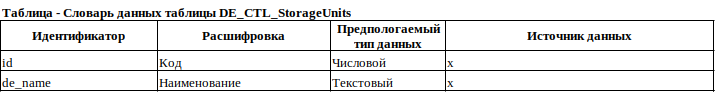
\includegraphics[width=16cm]
    {assets/InformationalModel/DE_CTL_StorageUnits.png}
    \caption{Словарь данных справочника <<Единицы хранения>>}
    \label{fig:InformationalModel_DE_CTL_StorageUnits}
\end{figure}

% \begin{table}[h!]
%     \centering
% 
%     \scriptsize
% 
%     \caption{Словарь данных справочника <<Единицы хранения>>}
% 
%     \label{table:CPR_EdiniciXraneniya_tipi}
% 
%     \begin{tabular}{|M{0.7cm}|M{3.1cm}|M{5cm}|M{2cm}|M{5cm}|} 
%         \hline
%         \textbf{№ п/п}&\textbf{Идентификатор}&\textbf{Наименование}&\textbf{Тип данных и значность}&\textbf{Источник данных}\\ \hline
%     \end{tabular}
% 
%     \begin{tabular}{|M{0.7cm}|p{3.1cm}|p{5cm}|p{2cm}|p{5cm}|} 
%         \hline
%         1&id&Код&N16&\\ \hline
%         2&Наименование&Единица хранения&C64&\\ \hline
%     \end{tabular}
% \end{table}

% \begin{figure}[!h]
%     \centering
%     \includegraphics[width=14cm]
%         {_docs/СП_ЕдХран_типы.jpg}
%     \caption{Словарь данных справочника <<Единицы хранения>>}
%     \label{fig:CP_EdXran_tipi}
% \end{figure}

% \begin{figure}[!h]
%     \centering
%     \includegraphics[]
%         {_docs/СП_ЕдХран_макет.jpg}
%     \caption{Макет справочника <<Единицы хранения>>}
%     \label{fig:CP_EdXran_maket}
% \end{figure}

\subsubsection{Справочный документ <<Мои организации>>}

Справочник <<Мои организации>> - содержит информацию о моих организациях.
Документ представлен в виде словаря данных (см.~рисунок~\ref{fig:InformationalModel_DE_CTL_MyOrganization}).
%и макета (рисунок~\ref{fig:CP_MoiOrg_maket}).

\begin{figure}[!h]
    \centering
    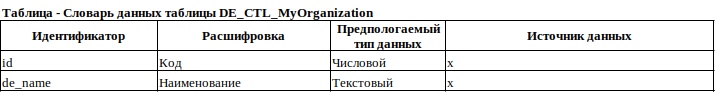
\includegraphics[width=16cm]
    {assets/InformationalModel/DE_CTL_MyOrganization.png}
    \caption{Словарь данных справочника <<Мои организации>>}
    \label{fig:InformationalModel_DE_CTL_MyOrganization}
\end{figure}

% \begin{table}[h!]
%     \centering

%     \scriptsize

%     \caption{Словарь данных справочника <<Мои организации>>}

%     \label{table:CPR_MoiOrganizatii_tipi}

%     \begin{tabular}{|M{0.7cm}|M{3.1cm}|M{5cm}|M{2cm}|M{5cm}|} 
%         \hline
%         \textbf{№ п/п}&\textbf{Идентификатор}&\textbf{Наименование}&\textbf{Тип данных и значность}&\textbf{Источник данных}\\ \hline
%     \end{tabular}

%     \begin{tabular}{|M{0.7cm}|p{3.1cm}|p{5cm}|p{2cm}|p{5cm}|} 
%         \hline
%         1&id&Код&N16&\\ \hline
%         2&Наименование&Название организации&C64&\\ \hline
%     \end{tabular}
% \end{table}

% \begin{figure}[!h]
%     \centering
%     \includegraphics[width=14cm]
%         {_docs/СП_МоиОрг_типы.jpg}
%     \caption{Словарь данных справочника <<Мои организации>>}
%     \label{fig:CP_MoiOrg_tipi}
% \end{figure}

% \begin{figure}[!h]
%     \centering
%     \includegraphics[]
%         {_docs/СП_МоиОрг_макет.jpg}
%     \caption{Макет справочника <<Мои организации>>}
%     \label{fig:CP_MoiOrg_maket}
% \end{figure}

\subsubsection{Справочный документ <<Производители>>}

Справочник <<Производители>> - содержит перечисление производителей.
Документ представлен в виде словаря данных (см.~рисунок~\ref{fig:InformationalModel_DE_CTL_Producers}).
% и макета (рисунок~\ref{fig:CP_Proizv_maket}).

\begin{figure}[!h]
    \centering
    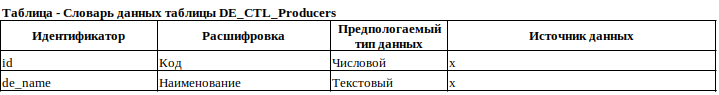
\includegraphics[width=16cm]
    {assets/InformationalModel/DE_CTL_Producers.png}
    \caption{Словарь данных справочника <<Производители>>}
    \label{fig:InformationalModel_DE_CTL_Producers}
\end{figure}

%\begin{table}[h!]
%    \centering
%
%    \scriptsize
%
%    \caption{Словарь данных справочника <<Производители>>}
%
%    \label{table:CPR_Proizvoditeli_tipi}
%
%    \begin{tabular}{|M{0.7cm}|M{3.1cm}|M{5cm}|M{2cm}|M{5cm}|} 
%        \hline
%        \textbf{№ п/п}&\textbf{Идентификатор}&\textbf{Наименование}&\textbf{Тип данных и значность}&\textbf{Источник данных}\\ \hline
%    \end{tabular}
%
%    \begin{tabular}{|M{0.7cm}|p{3.1cm}|p{5cm}|p{2cm}|p{5cm}|} 
%        \hline
%        1&id&Код&N16&\\ \hline
%        2&Наименование&Производитель номенклатуры&C64&\\ \hline
%    \end{tabular}
%\end{table}

% \begin{figure}[!h]
%     \centering
%     \includegraphics[width=14cm]
%         {_docs/СП_Произв_типы.jpg}
%     \caption{Словарь данных справочника <<Производители>>}
%     \label{fig:CP_Proizv_tipi}
% \end{figure}

% \begin{figure}[!h]
%     \centering
%     \includegraphics[]
%         {_docs/СП_Произв_макет.jpg}
%     \caption{Макет справочника <<Производители>>}
%     \label{fig:CP_Proizv_maket}
% \end{figure}

\subsubsection{Справочный документ <<Места хранения>>}

Справочник <<Места хранения>> - содержит перечисление адреса с номером склада.
Документ представлен в виде словаря данных (см.~рисунок~\ref{fig:InformationalModel_DE_CTL_StorageLocations}).
% и макета (рисунок~\ref{fig:CP_MestaXran_maket}).

\begin{figure}[!h]
    \centering
    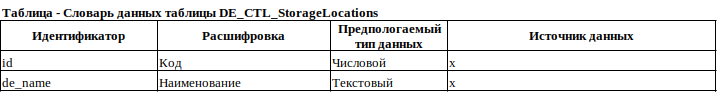
\includegraphics[width=16cm]
    {assets/InformationalModel/DE_CTL_StorageLocations.png}
    \caption{Словарь данных справочника <<Места хранения>>}
    \label{fig:InformationalModel_DE_CTL_StorageLocations}
\end{figure}

%\begin{table}[h!]
%    \centering
%
%    \scriptsize
%
%    \caption{Словарь данных справочника <<Места хранения>>}
%
%    \label{table:CPR_MestaXraneniay_tipi}
%
%    \begin{tabular}{|M{0.7cm}|M{3.1cm}|M{5cm}|M{2cm}|M{5cm}|} 
%        \hline
%        \textbf{№ п/п}&\textbf{Идентификатор}&\textbf{Наименование}&\textbf{Тип данных и значность}&\textbf{Источник данных}\\ \hline
%    \end{tabular}
%
%    \begin{tabular}{|M{0.7cm}|p{3.1cm}|p{5cm}|p{2cm}|p{5cm}|} 
%        \hline
%        1&id&Код&N16&\\ \hline
%        2&Наименование&Место хранения номенклатуры (адрес)&C64&\\ \hline
%    \end{tabular}
%\end{table}

% \begin{figure}[!h]
%     \centering
%     \includegraphics[width=14cm]
%         {_docs/СП_МестаХран_типы.jpg}
%     \caption{Словарь данных справочника <<Места хранения>>}
%     \label{fig:CP_MestaXran_tipi}
% \end{figure}

% \begin{figure}[!h]
%     \centering
%     \includegraphics[]
%         {_docs/СП_МестаХран_макет.jpg}
%     \caption{Макет справочника <<Места хранения>>}
%     \label{fig:CP_MestaXran_maket}
% \end{figure}

\newpage
\subsubsection{Оперативный документ <<Приказ о создании инвентаризационной комиссии>>}

Оперативный документ <<Приказ о создании инвентаризационной комиссии>>
- документ, который формируется перед инвентаризацией товара.
Документ представлен в виде словаря данных (см.~рисунки~\ref{fig:InformationalModel_DE_DOC_OrderCreationInventoryCommission} и \ref{fig:InformationalModel_DE_TAB_ListInventoryCommission}),
макета (см.~рисунок~\ref{fig:DOC_PrilazSozdInventKomis})
и схемы связей (см.~рисунок~\ref{fig:ARIS_GeneralDiagram_DOC_PrikazSozdInventKomis}).

\begin{figure}[!h]
    \centering
    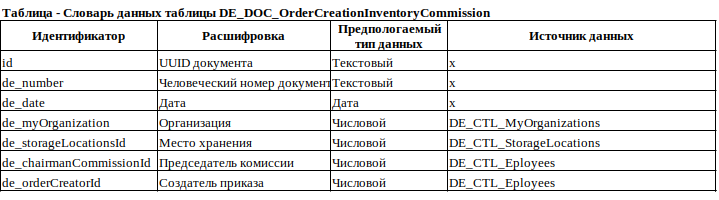
\includegraphics[width=16cm]
    {assets/InformationalModel/DE_DOC_OrderCreationInventoryCommission.png}
    \caption{Словарь данных оперативного документа <<Приказ о создании инвентаризационной комиссии>>}
    \label{fig:InformationalModel_DE_DOC_OrderCreationInventoryCommission}
\end{figure}

\begin{figure}[!h]
    \centering
    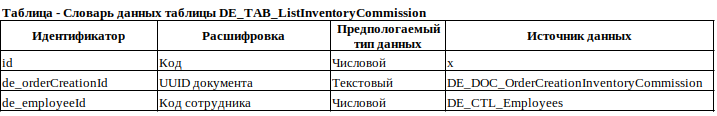
\includegraphics[width=16cm]
    {assets/InformationalModel/DE_TAB_ListInventoryCommission.png}
    \caption{Словарь данных табличной части <<Список членов инвентаризационной комиссии>>}
    \label{fig:InformationalModel_DE_TAB_ListInventoryCommission}
\end{figure}

% \begin{table}[h!]
%     \centering

%     \scriptsize

%     \caption{Словарь данных документа <<Приказ о создании инвентаризационной комиссии>>}

%     \label{table:DOC_PrikazCozdInventKomis}

%     \begin{tabular}{|M{0.7cm}|M{3.1cm}|M{5cm}|M{2cm}|M{5cm}|} 
%         \hline
%         \textbf{№ п/п}&\textbf{Идентификатор}&\textbf{Наименование}&\textbf{Тип данных и значность}&\textbf{Источник данных}\\ \hline
%     \end{tabular}

%     \begin{tabular}{|M{0.7cm}|p{3.1cm}|p{5cm}|p{2cm}|p{5cm}|} 
%         \hline
%         1&id&Автоинкримент&C128&\\ \hline
%         2&Номер&Номер документа&N8&\\ \hline
%         3&Дата&Дата проведения&TIME&\\ \hline
%         4&МоиОрганизацииId&Организация&N16&СПР\_МоиОрганизации\\ \hline
%         5&МестаХраненияId&Место хранения&N16&СПР\_МестаХранения\\ \hline
%         6&СотрудникиId\_Пред седательКомиссии&Гланый в комиссии&N16&СПР\_Сотрудники\\ \hline
%         7&СотрудникиId\_Созда тельПриказа&Сотрудник создавший приказ&N16&СПР\_Сотрудники\\ \hline
%     \end{tabular}
% \end{table}

% \begin{table}[h!]
%     \centering

%     \scriptsize

%     \caption{Словарь данных табличной части <<Список членов инвентаризационной комиссии>>}

%     \label{table:TAB_SpisokInventKomis}

%     \begin{tabular}{|M{0.7cm}|M{3.1cm}|M{5cm}|M{2cm}|M{5cm}|} 
%         \hline
%         \textbf{№ п/п}&\textbf{Идентификатор}&\textbf{Наименование}&\textbf{Тип данных и значность}&\textbf{Источник данных}\\ \hline
%     \end{tabular}

%     \begin{tabular}{|M{0.7cm}|p{3.1cm}|p{5cm}|p{2cm}|p{5cm}|} 
%         \hline
%         1&id&Автоинкримент&N16&\\ \hline
%         2&ПриказСоздИнвент КомисId&Код документа&C128&ДОК\_ПриказСоздИнвентКомис\\ \hline
%         3&СотрудникиId&Сотрудник&N16&СПР\_Сотрудники\\ \hline
%     \end{tabular}
% \end{table}

% \begin{figure}[!h]
%     \centering
%     \includegraphics[width=14cm]
%         {_docs/ОП_ПриказСоздКомИнвент_типы.jpg}
%     \caption{Словарь данных документа <<Приказ о создании инвентаризационной комиссии>>}
%     \label{fig:OP_PrikazSozdKomInvest_tipi}
% \end{figure}

\begin{figure}[!h]
    \centering

    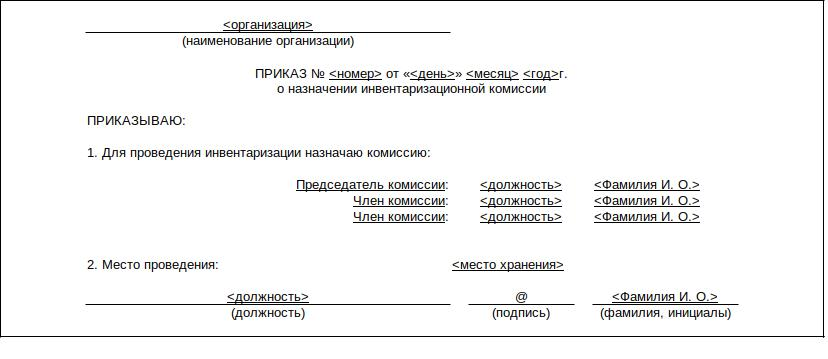
\includegraphics[width=17cm]
    {assets/layouts/DOC_PrilazSozdInventKomis.jpg}

    \caption{Макет документа <<Приказ о создании инвентаризационной комиссии>>}

    \label{fig:DOC_PrilazSozdInventKomis}
\end{figure}

\begin{figure}[!h]
    \centering
    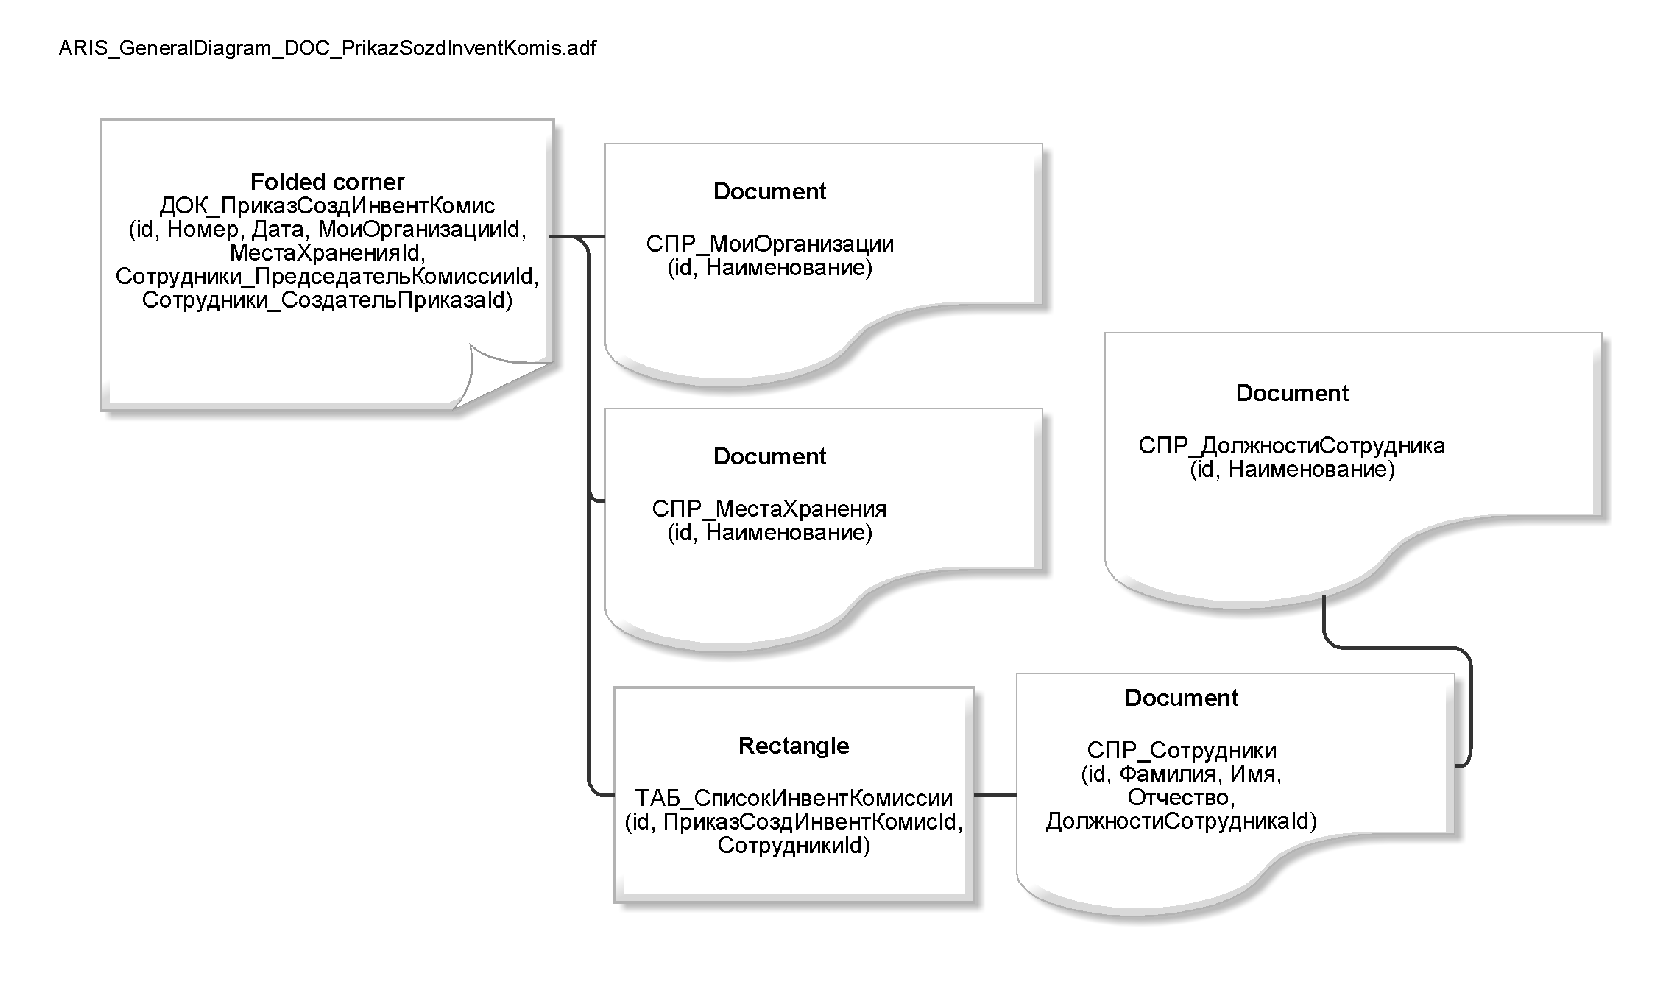
\includegraphics[width=14cm]
        {assets/ARIS/ARIS_GeneralDiagram_DOC_PrikazSozdInventKomis.adf.pdf}
    \caption{Схема информационной связи документа <<Приказ о создании инвентаризационной комиссии>>}
    \label{fig:ARIS_GeneralDiagram_DOC_PrikazSozdInventKomis}
\end{figure}

\newpage

\subsubsection{Оперативный документ <<Инвентаризационная опись>>}

Оперативный документ <<Инвентаризационная опись>>
- документ, в котором отображаются результаты инвентаризации.
Документ представлен в виде словаря данных (см.~рисунки~\ref{fig:InformationalModel_DE_DOC_InventoryList} и \ref{fig:InformationalModel_DE_TAB_NomenclatureInventList}),
макета (см.~рисунок~\ref{fig:DOC_InventOpis})
и схемы связей (см.~рисунок~\ref{fig:ARIS_GeneralDiagram_DOC_InventOpis}).

\begin{figure}[!h]
    \centering
    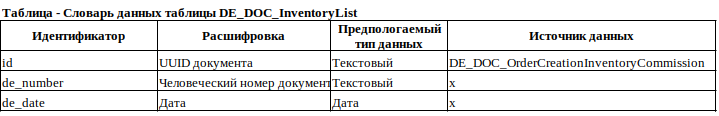
\includegraphics[width=16cm]
    {assets/InformationalModel/DE_DOC_InventoryList.png}
    \caption{Словарь данных оперативного документа <<Инвентаризационная опись>>}
    \label{fig:InformationalModel_DE_DOC_InventoryList}
\end{figure}

\begin{figure}[!h]
    \centering
    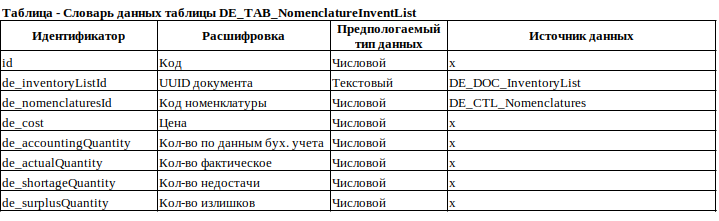
\includegraphics[width=16cm]
    {assets/InformationalModel/DE_TAB_NomenclatureInventList.png}
    \caption{Словарь данных табличной части <<Список номенклатуры инвентаризационной описи>>}
    \label{fig:InformationalModel_DE_TAB_NomenclatureInventList}
\end{figure}

% \begin{table}[h!]
%     \centering

%     \scriptsize

%     \caption{Словарь данных документа <<Инвентаризационная опись>>}

%     \label{table:DOC_InventOpis}

%     \begin{tabular}{|M{0.7cm}|M{3.1cm}|M{5cm}|M{2cm}|M{5cm}|} 
%         \hline
%         \textbf{№ п/п}&\textbf{Идентификатор}&\textbf{Наименование}&\textbf{Тип данных и значность}&\textbf{Источник данных}\\ \hline
%     \end{tabular}

%     \begin{tabular}{|M{0.7cm}|p{3.1cm}|p{5cm}|p{2cm}|p{5cm}|} 
%         \hline
%         1&id&UUID&C128&\\ \hline
%         2&Номер&Номер документа&N8&\\ \hline
%         3&Дата&Дата проведения&TIME&\\ \hline
%     \end{tabular}
% \end{table}

% \begin{table}[h!]
%     \centering

%     \scriptsize

%     \caption{Словарь данных табличной части <<Список номенклатуры инвентаризационной описи>>}

%     \label{table:TAB_SpisokInventKomis}

%     \begin{tabular}{|M{0.7cm}|M{3.1cm}|M{5cm}|M{2cm}|M{5cm}|} 
%         \hline
%         \textbf{№ п/п}&\textbf{Идентификатор}&\textbf{Наименование}&\textbf{Тип данных и значность}&\textbf{Источник данных}\\ \hline
%     \end{tabular}

%     \begin{tabular}{|M{0.7cm}|p{3.1cm}|p{5cm}|p{2cm}|p{5cm}|} 
%         \hline
%         1&id&UUID&N16&\\ \hline
%         2&ИнвентОписьId&Код документа&C128&ДОК\_ИнвентОпись\\ \hline
%         3&НоменклатураId&Номенклатура&N16&СПР\_Номенклатура\\ \hline
%         4&Цена&Цена номенклатуры&F8&\\ \hline
%         5&КоличПоДаннымБух Учёта&Количество по данным бухгалтерского учёта&N8&\\ \hline
%         6&КоличФактич&Количество фактическое&N8&\\ \hline
%         7&КоличНедосдачи&Количество недосдачи&N8&\\ \hline
%         8&КоличИзлишек&Количество излишек&N8&\\ \hline
%     \end{tabular}
% \end{table}

% \begin{figure}[!h]
%     \centering
%     \includegraphics[width=12cm]
%         {_docs/ОП_ИнвенОпис_типы.jpg}
%     \caption{Словарь данных документа <<Инвентаризационная опись>>}
%     \label{fig:OP_InvenOpis_tipi}
% \end{figure}

\begin{figure}[!h]
    \centering

    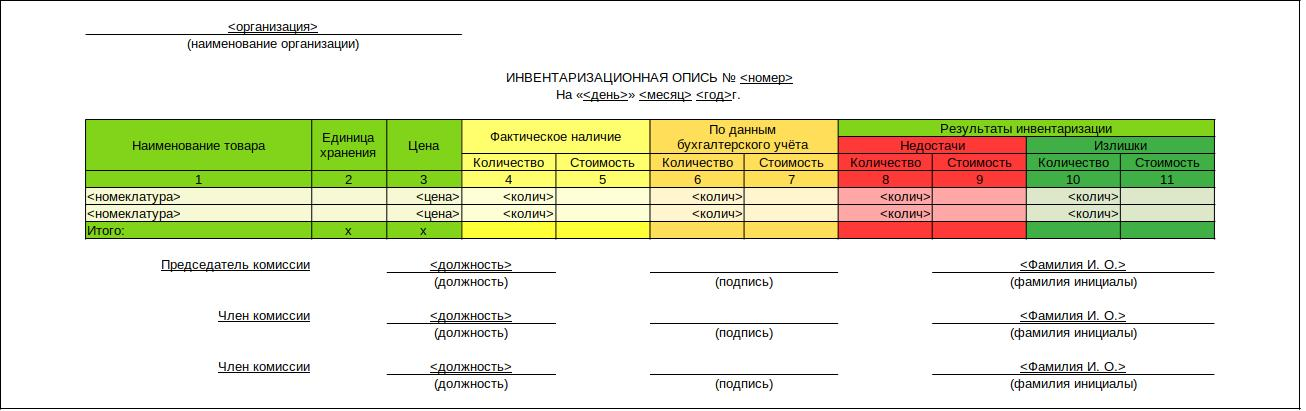
\includegraphics[width=17cm]
    {assets/layouts/DOC_InventOpis'.jpg}

    \caption{Макет документа <<Инвентаризационная опись>>}

    \label{fig:DOC_InventOpis}
\end{figure}

\begin{figure}[!h]
    \centering

    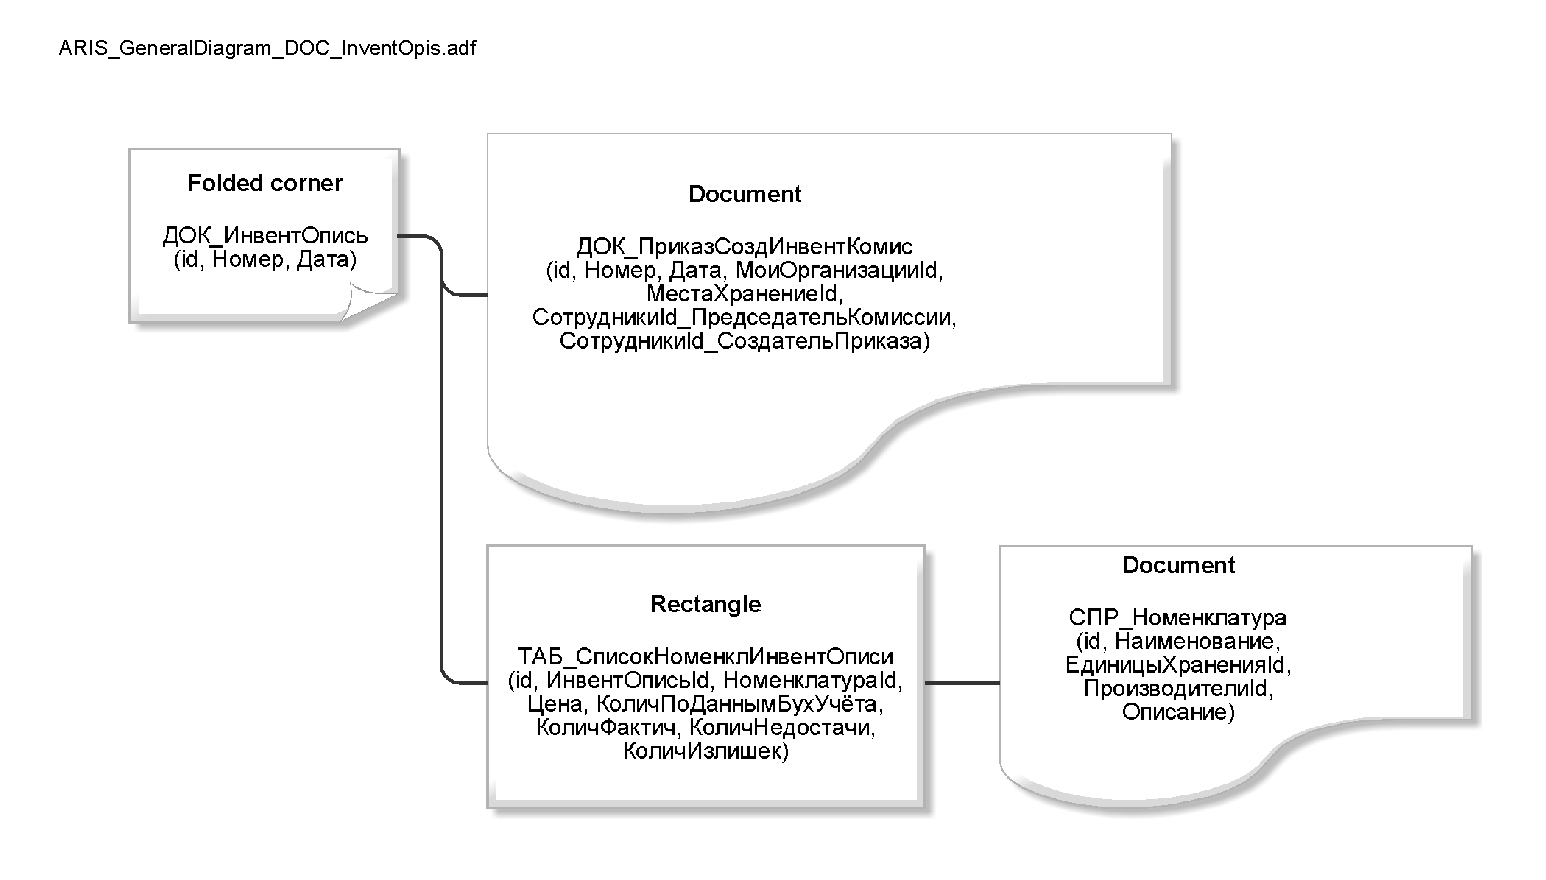
\includegraphics[width=11cm]
    {assets/ARIS/ARIS_GeneralDiagram_DOC_InventOpis.adf.pdf}

    \caption{Схема информационной связи документа <<Инвентаризационная опись>>}

    \label{fig:ARIS_GeneralDiagram_DOC_InventOpis}
\end{figure}

\newpage
\subsubsection{Отчёт <<Акт об инвентаризации>>}

Отчёт <<Акт об инвентаризации>>
- формируется после проведения инвентаризации (см. рисунок~\ref{fig:OTC_ActNedoctachiTovara}).
Состоит отчёт из данных двух документов:
\begin{itemize}
    \item <<Приказ о создании инвентаризационной комиссии>>;
    \item <<Инвентаризационная опись>>.
\end{itemize}

\begin{figure}[!h]
    \centering

    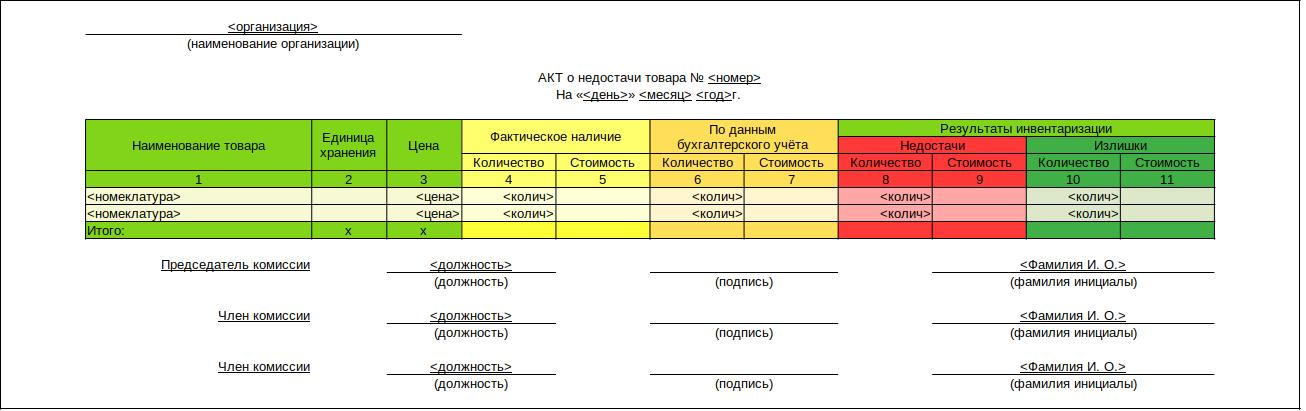
\includegraphics[width=17cm]
    {assets/layouts/OTC_ActNedoctachiTovara.jpg}

    \caption{Макет документа <<Инвентаризационная опись>>}
    
    \label{fig:OTC_ActNedoctachiTovara}
\end{figure}

% \begin{figure}[!h]
%     \centering
%     \includegraphics[width=14cm]
%         {_docs/ОТ_АктНедосТов_типы.jpg}
%     \caption{Словарь данных документа <<Акт о нестаче товара>>}
%     \label{fig:OT_AktNedosTov_tipi}
% \end{figure}

% \begin{figure}[!h]
%     \centering
%     \includegraphics[width=14cm]
%         {_docs/ОТ_АктНедосТов_макет.jpg}
%     \caption{Макет документа <<Акт о нестаче товара>>}
%     \label{fig:OT_AktNedosTov_maket}
% \end{figure}

% \begin{figure}[!h]
%     \centering
%     \includegraphics[height=6cm]
%         {_docs/ОТ_АктНедосТов_связи.png}
%     \caption{Схема информационной связи документа <<Акт о нестаче товара>>}
%     \label{fig:OP_AktNedosTov_svazi}
% \end{figure}

\newpage
\subsection{Модель бизнес-процесса объекта автоматизации}

\textbf{Процесс} - любая деятельность, в которой используются ресурсы для преобразования входов в выходы.
Зачастую представляет из себя совокупность взаимосвязанных и совершенных работ,
в которых результаты одной работы являются началом другой работы,
образуя цепочку внутрненних поставщиков и потребителей.

\textbf{Бизнес-процесс} - устойчивая и целенаправленная совокупность взаимосвязанных видов деятельности,
которая по определённой технологии преобразует входной сигнал в выходной, представляющий ценность для потребителя.

\textbf{eEPC} - нотация для проектирования бизнес-процессов.
Данная нотация ARIS представляет бизнес-процесс как цепочку событий и действий (функций).
Каждое действие инициализируется и завершается событием.

\begin{figure}[!h]
    \centering
  
    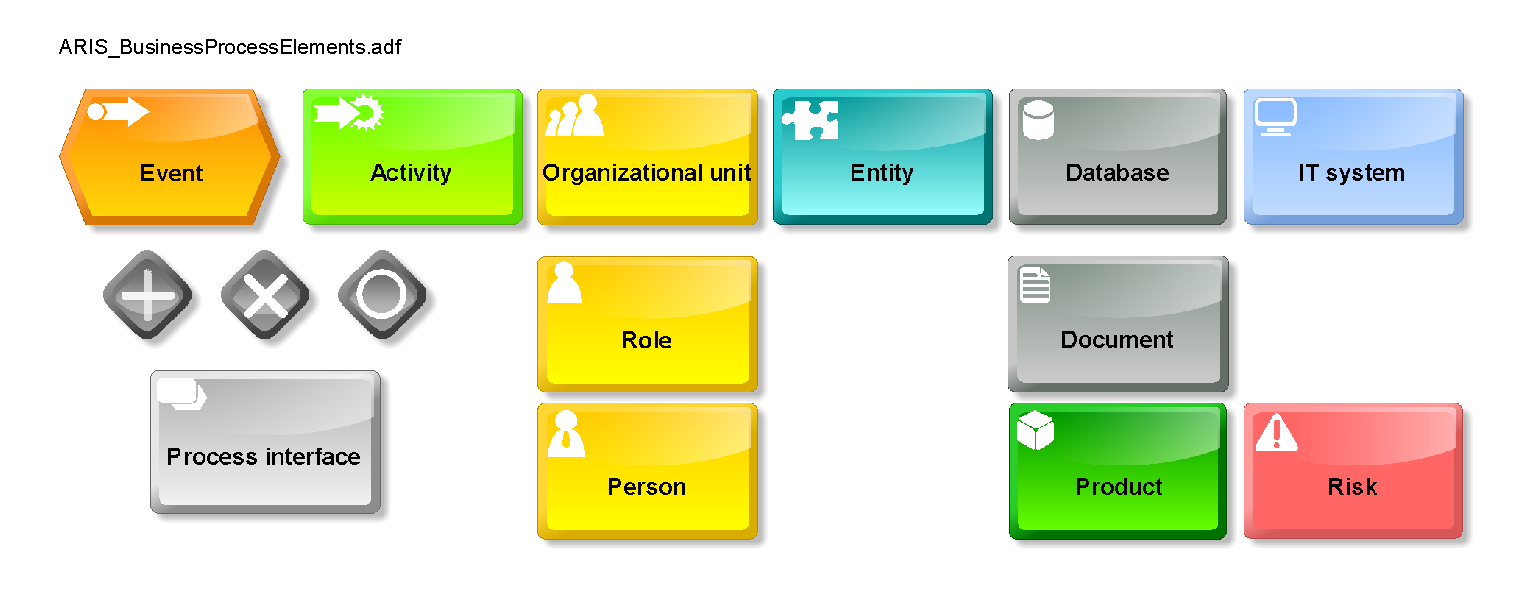
\includegraphics[height=6cm]
    {assets/ARIS/ARIS_BusinessProcessElements.adf.pdf}
    
    \caption{Элменты нотации ARIS Business Process}
    
    \label{fig:MBP_Product}
\end{figure}

\textbf{Event} - состояние, которое является существенным для целей управления бизнесом
и оказывает влияние или контролирует дальнейшее развитие одного или более бизнес-процессов.
Элемент отображает события, активизирующие функции или порождаемые функциями.
Внутри блока помещается наименование события.
Событие именуется отглагольным существительным.

\textbf{Activity} - действие или набор действий, выполняемых над исходным объектом с целью получения заданного результата.
Внутри блока помещается наименование функции (глагол или отглагольное существительное).
Временная последовательность выполнения функций задается расположением функций на диаграмме процесса сверху вниз.
Функция именуется глаголом или отглагольным существительным.

\textbf{Entity} - смысловая единица даталогической модели (модель «сущность-связь»)

\textbf{Document} - бумажный или электронный носитель информации.

\textbf{Product} - ресурс или услуга, используемый как для входа в функцию, так и как результат ее выполнения.

Модель бизнесс-процесса ОА <<Инвентаризация>> для ИС <<Косметический салон>> представлена нотацией ARIS Business Process
(см.~рисунок~\ref{fig:ARIS_BusinessProcess}).

\newpage

\begin{figure}[!h]
    \centering

    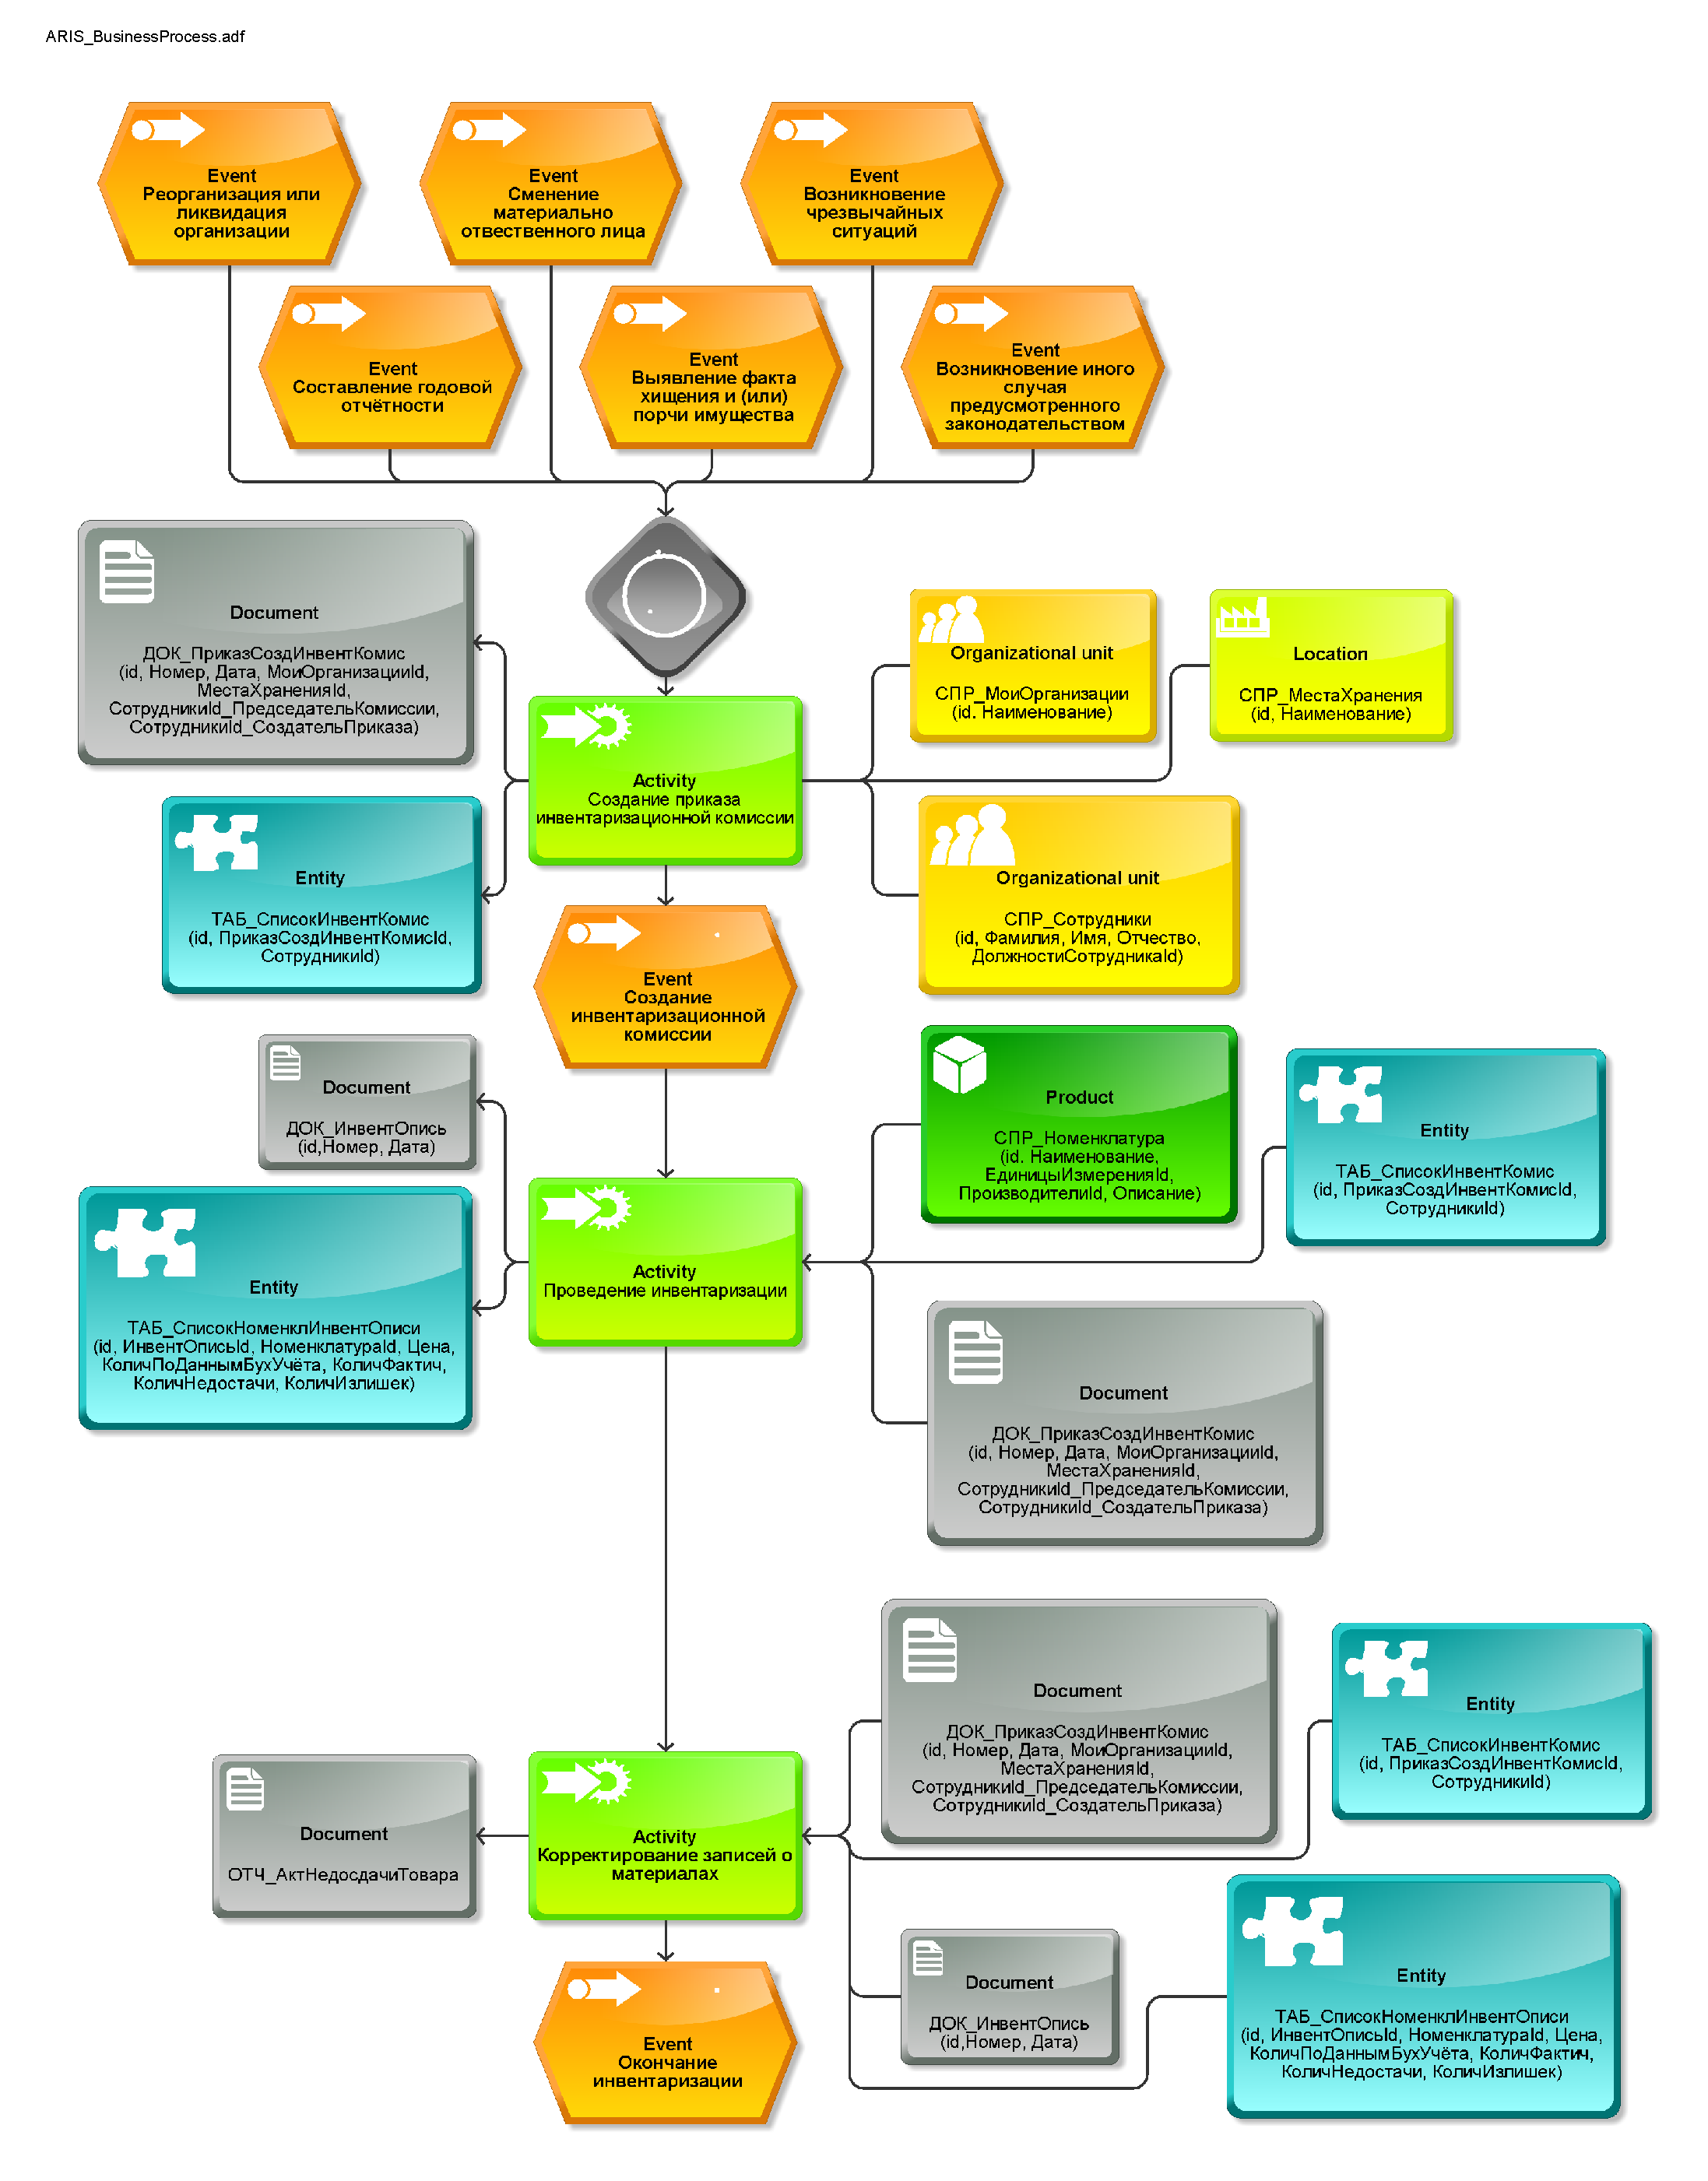
\includegraphics[width=18cm]
    {assets/ARIS/ARIS_BusinessProcess.adf.pdf}

    \caption{Модель БП ОА «Инвентаризация» для ИС <<Косметический салон>>}

    \label{fig:ARIS_BusinessProcess}
\end{figure}

\newpage
